%%%%%%%%%%%%%%%%%%%%%%%%%%%%%%%%%%%%%%%%%%%%%%%%%%%%%%%%%%%%

\section{Einführung}

Lorem ipsum dolor sit amet, consetetur sadipscing elitr, sed diam nonumy eirmod tempor invidunt ut labore et dolore magna aliquyam erat, sed diam voluptua. At vero eos et accusam et justo duo dolores et ea rebum. Stet clita kasd gubergren, no sea takimata sanctus est Lorem ipsum dolor sit amet. Lorem ipsum dolor sit amet, consetetur sadipscing elitr, sed diam nonumy eirmod tempor invidunt ut labore et dolore magna aliquyam erat, sed diam voluptua. At vero eos et accusam et justo duo dolores et ea rebum. Stet clita kasd gubergren, no sea takimata sanctus est Lorem ipsum dolor sit amet.

%%%%%%%%%%%%%%%%%%%%%%%%%%%%%%%%%%%%%%%%%%%%%%%%%%%%%%%%%%%%

\section{Verwandte Arbeiten}

Lorem ipsum dolor sit amet, consetetur sadipscing elitr, sed diam nonumy eirmod tempor invidunt ut labore et dolore magna aliquyam erat, sed diam voluptua \cite{ochmann-2014}. At vero eos et accusam et justo duo dolores et ea rebum \cite{ochmann-2014-towards}. Stet clita kasd gubergren, no sea takimata sanctus est Lorem ipsum dolor sit amet \cite{Ochmann-2015-Automatic}. Lorem ipsum dolor sit amet, consetetur sadipscing elitr, sed diam nonumy eirmod tempor invidunt ut labore et dolore magna aliquyam erat, sed diam voluptua. At vero eos et accusam et justo duo dolores et ea rebum. Stet clita kasd gubergren, no sea takimata sanctus est Lorem ipsum dolor sit amet.

%%%%%%%%%%%%%%%%%%%%%%%%%%%%%%%%%%%%%%%%%%%%%%%%%%%%%%%%%%%%

\section{Grundlagen}

Lorem ipsum dolor sit amet, consetetur sadipscing elitr, sed diam nonumy eirmod tempor invidunt ut labore et dolore magna aliquyam erat, sed diam voluptua. At vero eos et accusam et justo duo dolores et ea rebum. Stet clita kasd gubergren, no sea takimata sanctus est Lorem ipsum dolor sit amet. Lorem ipsum dolor sit amet, consetetur sadipscing elitr, sed diam nonumy eirmod tempor invidunt ut labore et dolore magna aliquyam erat, sed diam voluptua. At vero eos et accusam et justo duo dolores et ea rebum. Stet clita kasd gubergren, no sea takimata sanctus est Lorem ipsum dolor sit amet.

%%%%%%%%%%%%%%%%%%%%%%%%%%%%%%%%%%%%%%%%%%%%%%%%%%%%%%%%%%%%

\section{Aktionsklassifikation in VR}

Für die Klassifikation arbeiten wir im Gegensatz zu \cite{SceneGronk} nicht in realen Umgebungen, sondern verwenden virtuellen Szenen, in denen wir uns mit einer HTC Vive \cite{HTC-Vive} bewegen und den Szenenobjekten interagieren können. Dadurch können wir nicht nur einfacher verschiedene Umgebungen simulieren, sondern haben so auch die Möglichkeit mehr Informationen zu den Szenen und deren Objekten zu erhalten.
Für die Umsetzung haben wir ein Framework erstellt, das auf der Unreal Engine 4.14 \cite{UE4} aufbaut. Die Unreal Engine stellt die grundsätzlichen Funktionen, wie das Erstellen von Szenen und die Anbindung an die HTC Vive zur Verfügung. Das Framework erweitert die Funktionalität noch um das Aufnehmen und Abspielen von Aktionen, das Erstellen der Merkmalsvektoren aus diesen Aktionen \cite{Features} und der direkten Klassifizierung von neuen Aktionen.

\subsection{HTC Vive}
Für die Interaktion mit den virtuellen Szenen verwenden wir das VR-System HTC Vive. Zu dessen Umfang gehört ein Head-Mounted Display (HMD), zwei Controller und zwei Infarotsensoren. Diese sogenannten Basisstationen werden am Rand des zuvor festgelegten Feldes auf gegenüberliegenden Seiten aufgestellt und berechnen die Positionen und Orientierungen des HMDs, bzw. des Kopfs und der Controller bzw. den Händen. In diesem Feld kann sich der Benutzer frei bewegen und die Szenen durchlaufen. Um größere Distanzen zu überbrücken haben wir die Szenen so angepasst, dass man sich zu jeder Stelle teleportieren kann. Die HTC Vive bietet dank des Trackings von Kopf und Händen und der freien Bewegung im Raum schon eine gute Flexibilität, allerdings sind von den Posen des Nutzers so auch ohne Weiteres nur diese Positionen bekannt. Das Erkennen aller Gelenke wie in \cite{SceneGronk} ist so nicht möglich. \cite{FutureWork}

\subsection{Szenen}
Die Szenen werden mit U

\subsection{Kalibrierung}
Damit die ausgeführten Aktionen unabhängig von der Statur des Benutzers bleiben, wird vor der Aufnahme und Klassifizerung dessen Größe und Armlänge ermittelt. Dafür wird bei aufrechtem Stand und ausgestreckten Armen die Höhe des HMDs und dessen Abstand zu den Controllern gemessen. Diese Informationen werden mit jeder Aufnahme gespeichert und der Merkmalsberechnung zur Verfügung gestellt. 

\subsection{Aktionsaufnahme und Wiedergabe}
Der Benutzer startet die Aufnahme in einer Szene seiner Wahl und führt die gewünschte Aktion aus. Währendessen wird in regelmäßigen Abständen die aktuelle Position und Orientierung des HMDs, der Controller und jedes Szenenelements mitgeschrieben. Diese Informationen werden als Jsondokument gespeichert und können so auch leicht für andere Zwecke verwendet werden. Um gleiche Aktionen später gruppieren zu können, müssen deren Aufnahmen gleich benannt werden und dürfen sich im Namen nur um Zahlen unterscheiden.\newline
\begin{figure}[hbtp]
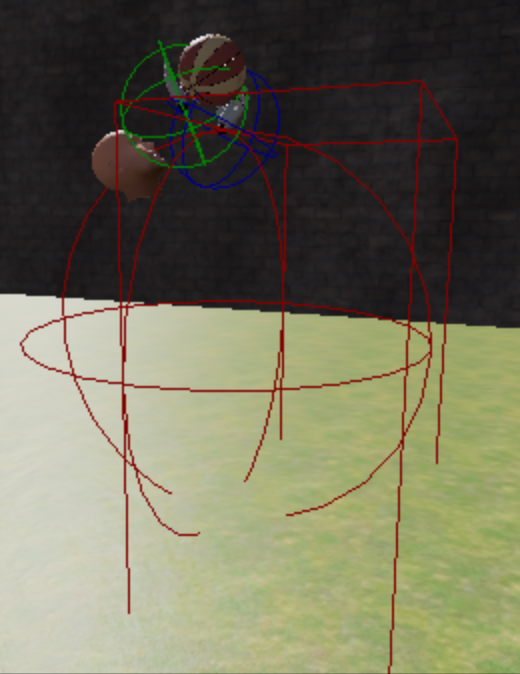
\includegraphics[height=0.3\textheight]{PlaybackActor.png}
\caption{Wiedergabe}
\label{fig:PlaybackActor}
\end{figure}
Bei der Wiedergabe werden das HMD und die Controller durch Modelle von Kopf und Händen dargestellt. Sie besitzen Hüllkörper mit denen die Gegenstände in der Nähe der Hände bzw. des Körpers ermittelt werden. Wir verwenden für die Hände Kugeln und für den Körper eine Halbkugel die vom Kopf senkrecht nach unten verläuft (Siehe Abb. \ref{fig:PlaybackActor}). Die Radien sind über die Einstellungen anpassbar. Zudem können bei der Wiedergabe zugleich die Merkmalsvektoren mit berechnet werden.

\subsection{Mermalsvektoren erstellen}
Welche Merkmale verwendet werden sollen wird im Quelltext angegeben. Die Unreal Engine bietet mit den sogenannten Blueprints eine graphenbasierte Alternative zur C++-Programierung an \cite{Blueprints}. Die von uns erstellte Blueprintfunktion "logFeatures" hat als Inputparameter die Kalibrierungsdaten, alle Informationen zu Kopf und Händen und einen Array mit den Featurevektoren, an den jeder neu Berechnete angehangen wird. Ein kurzes Beispiel ist in Abbildung \ref{fig:LogFeatures} zu sehen. Dort werden als Merkmale die Höhe des Kopfes und dessen Abstände zu den beiden Händen berechnet. Die von uns verwendeten Mermale werden in \cite{Features} genauer beschrieben. 
\begin{figure}[hbtp]
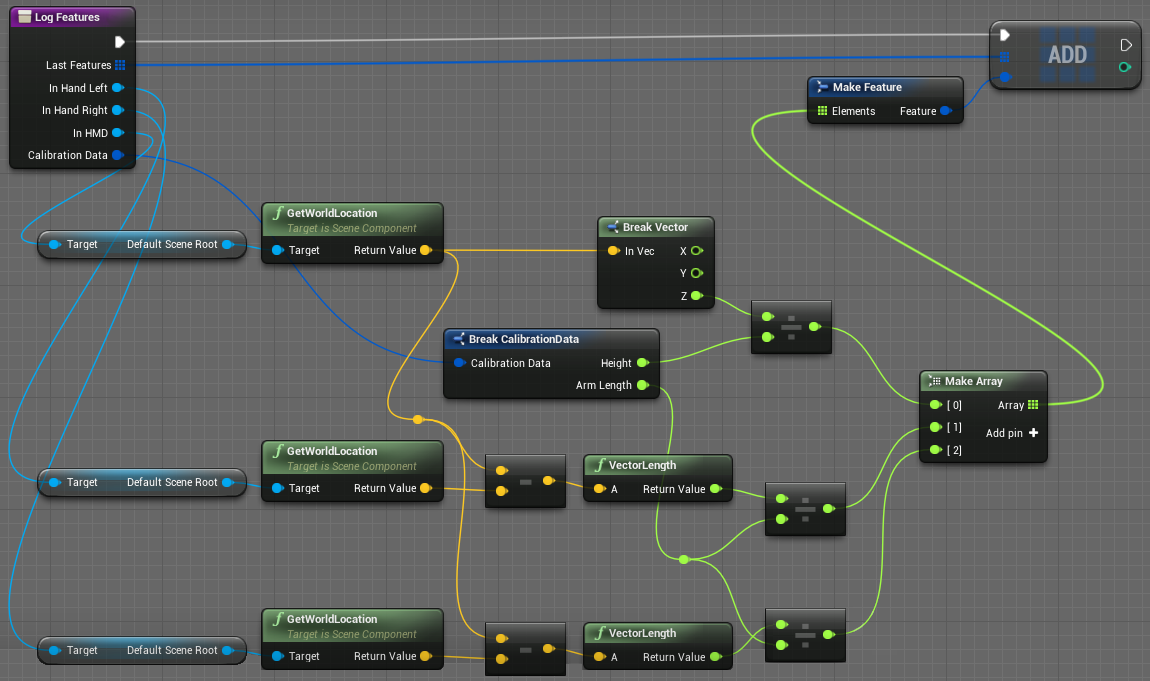
\includegraphics[width=1\linewidth]{LogFeatures2.png}
\caption{Merkalsvektoren im Blueprint erstellen}
\label{fig:LogFeatures}
\end{figure}

\subsection{Trainings- und Testdaten erstellen}
Die Trainings- und Testdaten werden außerhalb der Anwendung aus den aufgenommenen Merkmalsvektoren erstellt. Ein Skript gruppiert die Aufnahmen nach der Aktion und fügt die Hälfte der Aufnahmen jeder Gruppe in einer Testdatei und die andere Hälfte in einer Trainingsdatei zusammen. Aus den Trainingsdaten erstellt die Support-Vector-Machine libsvm \cite{libsvm} im Anschluss ein Trainingsmodell, auf dessen Grundlage die Klassifizierung der Test- bzw. Livedaten erfolgt.

\subsection{Live Klassifizierung}
Bei der Live Klassifizierung werden vom Benutzer Aktionen ausgeführt und daraus in Echtzeit die Featurevektoren bestimmt. Die Klassifizierung übernimmt die Bibliothek libsvm \cite{libsvm}, die über C++ an das Framework angebunden ist. Dafür werden zunächst aus den Merkmalsvektoren der Trainingsaufnahmen das Klassifizierungsmodell erstellt und vor der Live Klassifizierung eingelesen. Während der Klassifizierung wird dann jeder Featurevektor an die Support-Vector Machine weitergereicht, die auf der Grundlage des trainierten Modells die dargestellte Aktion prognostiziert. 


%%%%%%%%%%%%%%%%%%%%%%%%%%%%%%%%%%%%%%%%%%%%%%%%%%%%%%%%%%%%

\section{Evaluation und Resultate}

Lorem ipsum dolor sit amet, consetetur sadipscing elitr, sed diam nonumy eirmod tempor invidunt ut labore et dolore magna aliquyam erat, sed diam voluptua. At vero eos et accusam et justo duo dolores et ea rebum. Stet clita kasd gubergren, no sea takimata sanctus est Lorem ipsum dolor sit amet. Lorem ipsum dolor sit amet, consetetur sadipscing elitr, sed diam nonumy eirmod tempor invidunt ut labore et dolore magna aliquyam erat, sed diam voluptua. At vero eos et accusam et justo duo dolores et ea rebum. Stet clita kasd gubergren, no sea takimata sanctus est Lorem ipsum dolor sit amet.

%%%%%%%%%%%%%%%%%%%%%%%%%%%%%%%%%%%%%%%%%%%%%%%%%%%%%%%%%%%%

\section{Ausblick}

Lorem ipsum dolor sit amet, consetetur sadipscing elitr, sed diam nonumy eirmod tempor invidunt ut labore et dolore magna aliquyam erat, sed diam voluptua. At vero eos et accusam et justo duo dolores et ea rebum. Stet clita kasd gubergren, no sea takimata sanctus est Lorem ipsum dolor sit amet. Lorem ipsum dolor sit amet, consetetur sadipscing elitr, sed diam nonumy eirmod tempor invidunt ut labore et dolore magna aliquyam erat, sed diam voluptua. At vero eos et accusam et justo duo dolores et ea rebum. Stet clita kasd gubergren, no sea takimata sanctus est Lorem ipsum dolor sit amet.

%%%%%%%%%%%%%%%%%%%%%%%%%%%%%%%%%%%%%%%%%%%%%%%%%%%%%%%%%%%%
